\section{Rilevamento rumore ambientale}
Il microfono viene utilizzato per identificare un'eccessiva soglia di rumore nell'ambiente. Come per il precedente utilizzo dei sensori sono state definiti tre livelli di sensibilità ciascuno dei quali fa riferimento ad uno specifico valore di decibels.

\begin{itemize}
	\item \texttt{LOW}: \texttt{NOISE\_THRESHOLD = 60}
	\item \texttt{MEDUM}:  \texttt{NOISE\_THRESHOLD = 50}
	\item \texttt{HIGH}:  \texttt{NOISE\_THRESHOLD = 30}
\end{itemize}

Per permettere all'utente di comprendere le operazioni in corso nell'applicazione viene mostrata una vista che contiene in valori in decibel campionati dal microfono. I valori sono rappresentati utilizzando un indicatore a doppio canale (in caso di dispositivi che supportano acquisizione stereo). Due livelli sono messi in risalto dall'indicatore, il primo è il valore di threashold oltre al quale viene segnalata un'intrusione mentre il secondo è una soglia arbitraria di rumore.

\begin{figure}[!ht]
\begin{center}
\makebox[\linewidth]{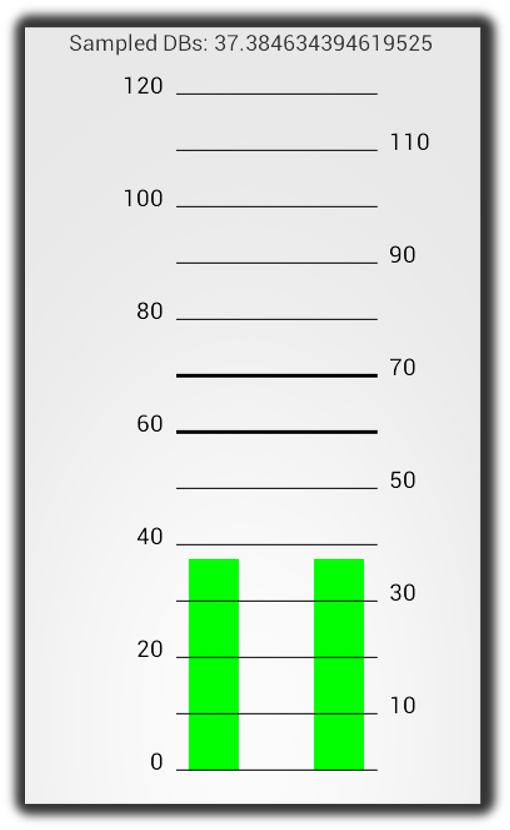
\includegraphics[scale=0.3]{../wireless/resources/microphone.png}}
\caption{Microphone view to show sampled audio level}
\label{img:microphone}
\end{center}
\end{figure}

\section{\textbf{Alert communication}}
If a user is logged in, different ways of alert communication have been implemented depending on the connectivity currently available:\\
\begin{itemize}
	\item \texttt{WIFI CONNECTIVITY}: a set of 10 captured images and 10 seconds of audio are sent
	\item \texttt{3G CONNECTIVITY}: a subset of 5 captured images and 10 seconds of audio are sent
	\item \texttt{BLUETOOTH CONNECTIVITY}: no images or audio are sent but bluetooth is used to opportunistically and periodically request other devices to send phone's position
\end{itemize}

In both cases of \texttt{WIFI} or \texttt{3G CONNECTIVITY} a periodic task is used to send phone's location to the back-end.

\subsection{Campionamento}
L'applicazione continua a campionare dal microfono un buffer di \texttt{512} valori in \texttt{PCM} a \texttt{16 BIT}.
Le \texttt{API} di Android permettono inoltre di campionare con \texttt{PCM 8 BIT}, al fine di ottenere una maggiore qualità del suono acquisito e considerando che tali valori non vanno salvati su disco su è adottata \texttt{PCM 16 BIT}.\\
Il microfono viene inoltre campionato in modalità mono di default, eventuali dispositivi che offrano microfoni audio in stereo sono campionati in stereo.\\

I valori ottenuti rappresentano la digitalizzazione del rumore ambientale. Al fine di rendere tali valori comprensibili per l'utente finale e di utilizzarli per identificare eventuali intrusioni è necessario convertirli in una misura di intensità. La letterature scientifica infatti offre un notevole numero di tabelle che mostrano per ciascun rumore comune il corrispondente valore in decibel, come in figura \ref{img:decibels}. 

\begin{figure}[!ht]
\begin{center}
\makebox[\linewidth]{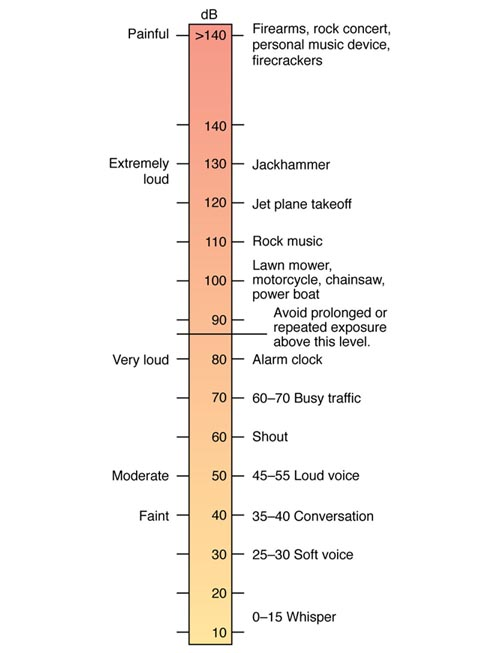
\includegraphics[scale=0.5]{../wireless/resources/decibels.jpeg}}
\caption{A decibel scale}
\label{img:decibels}
\end{center}
\end{figure}

Al fine quindi di sfruttare le informazioni contenute in queste tabelle e la maggior comprensibilità di valori in decibels i valori in \texttt{PCM 16 BIT} sono convertiti per ottere valori in \texttt{dB}.\\

Facendo riferimento ad una misura di ampiezza possiamo definire in decibel un valore $V_i$ rispetto ad un valore di riferimento $V_o$ come 20 volte il logaritmo in base dieci del rapporto quadratico, ovvero:

\begin{equation}
dB_i = 20log_{10} \left(\frac{V_i}{V_o}\right)
\end{equation}

Nella conversione dei valori \texttt{PCM} in valori in \texttt{dB} possiamo correttamente assumere che qualsiasi valore campionato dal microfono (valore \texttt{PCM} $\neq 0$) rappresente qualcosa di udibile. Con questa assunzione possiamo utilizzare il valore \texttt{1} come soglia di riferimento per il calcolo dei decibel.\\

Dato un campione sotto forma di array di \texttt{512 short integers} (che chiamiamo \texttt{signal}) lo pseudo-codice seguente può essere utilizzato per calcolare l'intensità media in \texttt{dB}:

\begin{lstlisting}[language=Java, caption=Pseudocode for computing dB from PCM samples]
int total = 0
int count = 0
for (short peak : signal) {
	if (peak != 0) {
		total=total+|peak|
		count=count+1
	}
}
int average = 0
if (count > 0) average = total/count

double averageDB = 0.0
if (average!=0) {
	averageDB = 20*log10((average)/1)
}
\end{lstlisting}

Il codice appena presentato calcola il valore medio dei moduli dei valori dei singoli campionamenti \texttt{PCM}, questo valore viene utilizzato per calcolare l'intensità in \texttt{dB} rispetto al valore di riferimento \texttt{1}.

\subsection{Registrazione}
Qualora fosse identificata un'intrusione viene avviato un \texttt{thread} che inizia l'acquisizione di 10 secondi di audio che saranno poi caricati sul server.\\

L'aquisizione avviene in formato \texttt{MPEG-4}.\\

\texttt{MPEG-4 - part 3} è la sezione dello standard che si occupa di audio e rappresenta un insieme di algoritmi di compressione tra cui \texttt{AAC} ed alcune sue variazioni.\\

\texttt{AAC} è uno schema di \textit{encoding} audio standardizzato definito per essere il successore di \texttt{MP3} (in effetti in generale raggiunge migliori qualità audio a parità di bit rate\footnote{Brandenburg, Karlheinz (1999). "MP3 and AAC Explained"}). \texttt{ACC} viene supportato nativamente dai dispositivi Android ed è per questo stato scelto schema di \textit{encoding}.\\

\fcolorbox{red!50!yellow}{red!20!yellow!50}{\parbox{\textwidth}{
  \vskip10pt
  \leftskip10pt\rightskip10pt
  \textbf{Note: Android audio encoding}\\
Il formato di encoding \texttt{MP3} non è reso disponibile per l'acquisizione da Android. Le ragioni sembrerebbero essere problematiche relative alla licenza. Negli anni infatti si sono susseguite diverse rivendicazioni di diritti sulle licenze necessarie per la produzione di audio in formato \texttt{MP3} risultando in molta confusione su cosa si possa o non si possa fare con il formato \texttt{M3}.\\

\texttt{AAC} invece non necessita di licenze per la riproduzione e la distribuzione di contenuti nel proprio formato.\\

Nonostante l'esistenza di alternative non licenziate come \texttt{Vorbis} queste non sono offerte dal sistema Android.
	
  \vskip10pt
 }
}\\

\texttt{AAC} opera secondo le seguenti fasi:

\begin{enumerate}
	\item Il segnale è convertito dal dominio del tempo al dominio della frequenza usando la trasformata coseno discreta modficata (\texttt{MDCT}). Questo viene fatto applicando banchi di filtri che prendono un numero appropriato di campioni nel tempo e li convertono a campioni di frequenza
	\item Il segnale nel dominio della frequenza viene quantizzato secondo il modello psicoacustico e codificato
	\item Sono applicati codici di correzione errori
	\item Il segnale viene salvato
\end{enumerate}

L'audio registrato e compresso utilizzando \texttt{AAC} viene poi trasmesso al back-end.

\subsection{Riproduzione}
Come detto l'audio catturato viene inviato all'applicazione web che deve provvedere alla riproduzione.\\
Per ragioni della semplicità implementativa la ripoduzione dell'audio viene effettuata sfruttando il tag \texttt{HTML5 <audio></audio>}.\\
I \texttt{MIMET Type} ammessi dal tag \texttt{<audio></audio>} e relativi formati sono i seguenti:

\begin{itemize}
	\item \texttt{audio/mpeg}: formato \texttt{MP3}
	\item \texttt{audio/mp4}: formato \texttt{AAC}
	\item \texttt{audio/ogg}: formato \texttt{Ogg Vorbis}
	\item \texttt{audio/wav}: formato \texttt{WAV}
\end{itemize}

La codifica con cui l'audio viene catturato è \texttt{AAC}, tuttavia nonstante questa sia ammessa non è supportata da tutti i browser:

\begin{center}
\begin{tabular}{ l c r }
\textbf{Browser} & \textbf{Version} & \textbf{Codec supportati} \\
\toprule
Internet Explorer &	9.0+ & MP3, AAC \\
\midrule
Chrome & 6.0+ & Ogg Vorbis, MP3, WAV \\
\midrule
Firefox & 3.6+ & Ogg Vorbis, WAV \\
\midrule
Safari & 5.0+ & MP3, AAC, WAV \\
\midrule
Opera & 10.0+ & Ogg Vorbis, WAV \\
\bottomrule
\end{tabular}
\end{center}

Come abbiamo visto non era possibile salvare diversamente l'audio e comunque non ci sono formati supportati da tutti i browser. Al fine di garantire una totale copertura si è deciso di scegliere le due codifice \texttt{AAC} e \texttt{Ogg Vorbis}.\\

La conversione direttamente su dispositivo da \texttt{AAC} a \texttt{Ogg Vorbis} è stata immediatamente esclusa:
\begin{itemize}
	\item Android non sembra supportare nativamente \texttt{Ogg Vorbis} ed inoltre effettuare questa conversione a livello applicazione Java risulterebbe eccessivamente oneroso
	\item Si dovrebbe trasmettere il file audio attraverso la rete in duplice formato
\end{itemize}
Da qui quindi la scelta di convertire nella codifica \texttt{Ogg Vorbis} nell'applicazione web in seguito al caricamento dell'audio.\\

La codifica \texttt{Vorbis} opera come:
\begin{enumerate}
	\item Utilizzo della trasformata coseno discreta modificata (\texttt{MDCT}) per passare al dominio delle frequenze
	\item Il dominio delle frequenze risultante viene suddiviso in \textit{noise floor} e residuo
	\item Il dominio delle frequenze viene poi quantizzato e compresso entropicamente
\end{enumerate}

La tecnica \textit{noise floor} conferisce a \texttt{Ogg Vorbis} la caratteristica di degradare verso un rumore simil-analogico quando il bit-rate non è sufficiente a riprodurre con qualità l'audio.\\

La conversione da \texttt{AAC} a \texttt{Ogg Vorbis} viene fatta avviando un processo corrispondente all'esecuzione del comando:\\

\begin{center}
	\texttt{ffmpeg -i in.m4a -acodec libvorbis -aq 60 -vn -ac 2 out.ogg}
\end{center}

\begin{itemize}
	\item \texttt{-i}: indica il nome del file di input
	\item \texttt{-acodec}: indica il codec da utilizzare per la conversione (\texttt{libvorbis})
	\item \texttt{-aq}: permette di specificare la qualità richiesta in caso di codec \texttt{VBR (Variable Bit Rate)}, ovvero codec che permettono di specificare una qualità attesa e che utilizzeranno qualsiasi bit rate per raggiungerla (\texttt{Ogg Vorbis} è uno di questi. 60 è una buona qualità nel nostro caso
	\item \texttt{-vn}: disabilita il video
	\item \texttt{-ac}: specifica il numero di stream audio, impostiamo 2 per supportare flussi stereo
\end{itemize}
